\chapter{Theorie}
\label{cha:Theorie}

\section{Eigenschaften der Myonen}

Myonen sind Leptonen und gehören zusammen mit den Myon-Neutrinos und entsprechenden Antiteilchen zu den Leptonen der zweiten Teilchengeneration des Standardmodells.
Sie haben eine Ruheenergie von $m_{\mu} \approx \qty{105.66}{\mega\electronvolt}/\mathrm{c}^2$\cite{PDG} und somit eine höhere Masse als Elektronen mit $m_{\mathrm{e}} 
\approx \qty{510.99}{\kilo\electronvolt}/\mathrm{c}^2$\cite{PDG}. Experimentell wurde eine mittlere Lebensdauer von $\tau(\mu^{\pm}) = \qty{2.1969e-6}{s} $ \cite{PDG} für das Myon bestimmt.\\
Beinahe alle $(\approx 100 \%)$ Myonen zerfallen über folgenden Zerfallskanal\cite{PDG}:
\begin{align}
    \mu^{-} &\rightarrow \mathrm{e}^{-} \bar{\nu}_{\mathrm{e}}\nu_{\mu} \\
    \mathrm{bzw.} \ \mu^{+} &\rightarrow \mathrm{e}^{+}\nu_{\mathrm{e}} \bar{\nu}_{\mu}.
\end{align}
Auf der Erde ist die größte Quelle für Myonen hochenergetische geladene kosmische Hadronen, welche beim Eindringen in die Erdatmosphäre Teilchenkaskaden auslösen. 
Diese Kaskaden bestehen aus hadronischen, elektromagnetischen und myonischen Komponenten. Letztere entstehen zum Großteil aus dem Zerfall geladener Pionen, welche
eine sehr kurze mittlere Lebendauer von $\tau_{\pi^{\pm}} \approx \qty{2.6e-8}{\second}$\cite{PDG} aufweisen und unteranderem über
\begin{align}
    \pi^{-} &\rightarrow \mu^{-} \bar{\nu}_{\mu} (\gamma)\\
    \mathrm{bzw.} \ \pi^{+} &\rightarrow \mu^{+} {\nu}_{\mu} (\gamma)
\end{align}
zu Myonen zerfallen. Bei den Zerfällen wird zumeist zusätzliche Energie mittels Photonen $\gamma$ abgestrahlt. Eine schematische Darstellung dieser Teilchenkaskaden ist in \autoref{fig:Teilchenshower}
dargestellt.\\
\begin{figure}
    \centering
    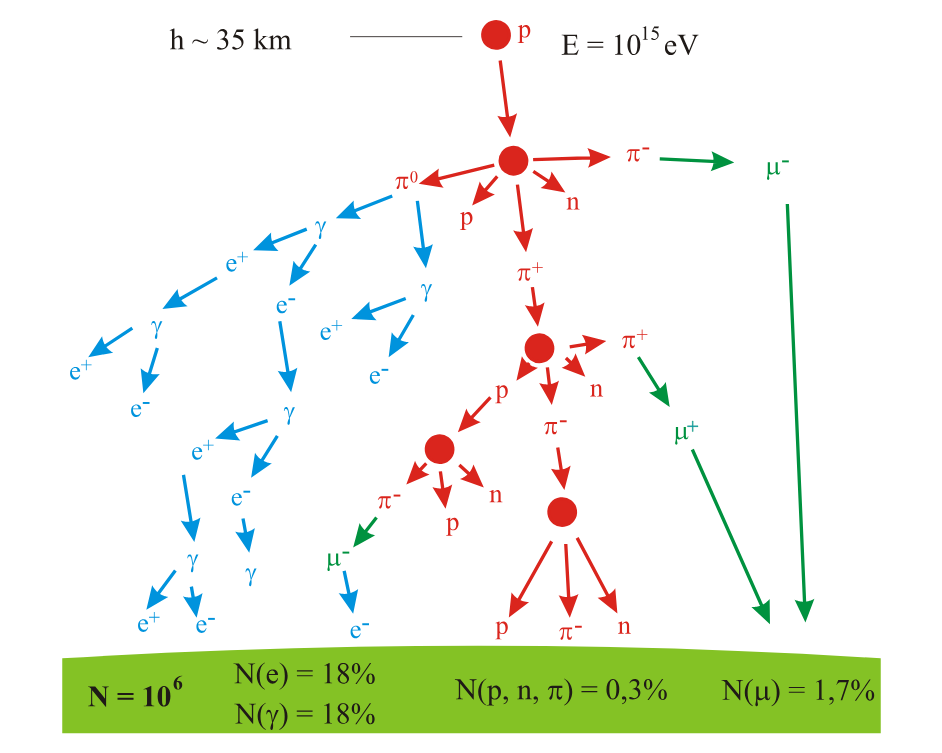
\includegraphics[width = 0.8\textwidth]{pics/Teilchenkaskade.png}
    \caption{. \cite{WikiKaskade}}
    \label{fig:Teilchenshower}
\end{figure}
Die kosmischen Myonen entstehen auf einer Höhe von etwa $\qty{10}{\kilo\meter}$\cite{MyonenAachen}. Obwohl diese Energien von einigen $\qty{}{\giga\electronvolt}$ besitzen und sich mit annähernd Lichtgeschwindigkeit
bewegen, zerfallen diese klassisch gerechnet nach einigen hundert Metern. Klassisch betrachtet würden die Myonen die Erdatmosphäre nicht erreichen. Durch die hohe Geschwindigkeit
muss eine relatvistische Rechnung angestellt werden und Effekte der Zeitdilatation berücksichtigt werden. Hier ergeben sich Reichweiten von mehr als $\qty{10}{\kilo\meter}$, bevor Myonen zerfallen.\\

\section{Mittlere Lebensdauer}

In diesem Versuch soll die Mittlere Lebensdauer von kosmischen Myonen experimentell untersucht werden. Die mittlere Lebensdauer von Teilchen gibt an, wie viel Zeit durchschnittlich vergeht, bevor
dieses zerfällt. Es handelt sich hierbei um den Erwartungswert der Verteilung der Lebensdauer, welcher im Folgenden hergeleitet wird.\\
In einem kleinen Zeitintervall sinkt die Anzahl der nicht zerfallenen Teilchen $N(t)$ mittels dem Zerfallsgesetz:
\begin{equation}
    \mathrm{d}N(t) = - \lambda N(t) \mathrm{d}t,
\end{equation}
wobei $\lambda$ eine Zerfallskonstante ist, welche spezifisch für den Zerfallskanal ist.\\
Ein lösen dieser Differentialgleichung und Integration führt zu einer exponentiellen Proportionalität
\begin{equation}
    N(t) = N_0 \exp{(-\lambda t)}.
\end{equation}
Für den Erwartungswert dieser Verteilung und schließlich der mittleren Lebensdauer ergibt sich schließlich
\begin{equation}
    \tau = \frac{1}{\lambda}.
\end{equation}

\section{Detektion kosmischer Myonen}

Die Myonen werden mittels eines Szintillatordetektors detektiert. Beim Eintritt eines Myons in den Szintillator wird ein Lichtimpuls an zwei Photomultiplier weitergeleitet. Hier werden mittels Photoeffekt
Elektronen herausgelöst, welche über ein elektrisches Feld zu einer Elektrode beschleunigt werden und weitere Elektronen herauslösen. Dieser Schritt wiederholt sich einige Male, bis ein starker Spannungspuls entsteht.
Die zwei Impulse aus den Photomultipliern werden über zwei Discriminator und zwei variable Delays in einen Coicidence geschickt. Da Photomultiplier durch thermische Strahlung zu spontanen Spannungspulsen neigen und 
ein Rauschen entsteht, soll mittels Discriminators dieses unterdrückt werden. Durch den Coicidence wird verhindert, dass fehlerhafte spontane Impulse als Signal registriert werden. Hier werden nämlich nur jene Impuls weitergeleitet,
welche an beiden Eingängen gleichzeitig ankommen. Es werden also nur jene Impuls akzeptiert, welche durch ein Event im Szintillator hervorgerufen wurden. Da die Impulse durch unterschiede in den Photomultipliern und Käbeln
verschiedene Verzögerungen bis zum Coincidence haben können, können diese durch variable Delays wieder korrigiert werden.\\
Aus dem Coicidence gehen schließlich drei verschiedene Kanäle aus. Ein Kanal unterläuft zunächst einen kurzen Delay von $\approx \qty{30}{\nano\second}$ und wird in einen Monoflop geleitet. Dieser wandelt das gepulste Signal in ein
durchgängiges Binärsignal um. Hier gibt es einen normalen und einen invertierten Ausgang. Ein Signal würde hier TRUE bedeutet und kein Signal FALSE. Der invertierte Ausgang des Monoflops wird zusammen mit einem der anderen beiden Kanäle des
Coincidence in eine AND-Logik geleitet, um ein Starten einer Stoppuhr zu triggern. Der normale Ausgang wird zusammen mit dem letzten Ausgang des Coincidence in eine andere AND-Logik geschaltet, welche ein Stoppen der Stoppuhr bewirken soll. 
Das Eintreten des Myons soll hier die Stoppuhr starten und ein zweiter Impuls beim Zerfall des Myons diese stoppen.\\
Der Delay vor dem Monoflop ist notwendig, damit die Signale bei den AND-Logiken nicht gleichzeitig ankommen. Hierdurch würde ein Starten oder Stoppen der Uhr nicht möglich sein.\\
Durch den Monoflop kann zudem eine Suchzeit eingestellt werden, nach der ein Event verworfen wird. Das ist sinnvoll für den Fall, dass ein Myon zu hochenergetisch ist, als dass es in dem Szintillatortank
zerfällt. Die Suchzeit ist so gewählt, dass sie etwa das 5-fache der erwarteten mittleren Lebensdauer beträgt.
\begin{figure}
    \centering
    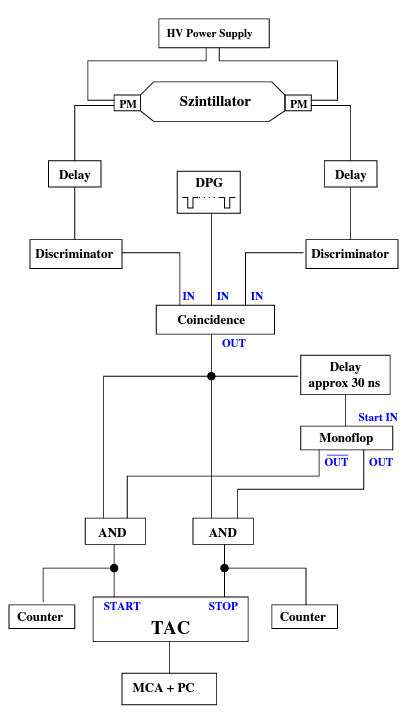
\includegraphics[width = 0.8\textwidth]{pics/Aufbau.png}
    \caption{. \cite{v01}}
    \label{fig:Aufbau}
\end{figure}